\chapter{Mathematical Background}\label{chapter:math}

Next, to address the practical part of the thesis, it is needed to give some attention to the underlying math. Considering that the system described in chapter \ref{chapter:implementation} extensively uses techniques and concepts from the field of digital signal processing, it was decided to make a brief introduction to the basics of it for a reader that might be confused by the variety of new terms. Thus, the present chapter will firstly describe how sound is represented computationally, and then will provide a few examples of the most common sounds. Next, a section dedicated to digital filters and filterbanks will follow, and finally, some other mathematical concepts used in the implementation part will be addressed.

\section{The Basics of Digital Signal Processing}\label{section:math_basics}

As it was described in chapter \ref{section:physics_sound}, physical sounds in real world spread in the environment in a form of pressure waves. These waves are continuous, thus to be able to work with sound via computers is it usually useful to convert them to some kind of a discrete representation. The notion of a discrete signal is used here and is defined as a time series sampled at equally-spaced points on the time axis. The term of sampling frequency $f_s$ is applicable, referring to the number of samples observed during a unit of time (the corresponding period is notated as $T_s$). Sometimes, discrete signals are represented as functions (for example, $x(n)$), or as vectors \cite{Abood2020}: $$\textbf{x} = [x(0), x(1), \dots{}, x(N - 1)]^T, \textbf{x}\in\mathbb{R}^N$$ where $N$ is overall number of samples.\\

If you recall the conversation about resonant frequencies and the sinusoidal manner of vibrations from chapter \ref{section:physics_sound}, you may remember that when an impulse is delivered to an object, the object responds to it by entering into vibrations. It starts to vibrate at all possible frequencies, but not all of them survive. An important mathematical instrument for frequency analysis is Fourier transform (along with Fourier series). Fourier theorem states that any periodic function might be represented as a sum of sines and cosines, so technically, any waveform of a sound (including the ones for sound waves) might be decomposed and represented in such a way. This decomposition may also be called amplitude spectrum, or spectral density.\\

The most basic example of such frequency decomposition is for a pure tone (the first row on figure \ref{img:windowing_example}). Pure tones are impossible to find in nature, or even perfectly produce with a speaker. Pure tones produced computationally sound flat and unnatural, but they are the basic building blocks of other sounds. The waveform of a pure tone is a sine wave and is defined as a function of time $t$: $$y(t) = A\sin(2\pi{}ft + \varphi),$$ where $f$ is frequency, $A$ is amplitude and $\varphi$ is phase. The frequency decomposition of a pure tone will contain only one peak at frequency $f$.\\

Another example of a common sound would be a click. Clicks are instant modulations in amplitude of a sound waveform, or waves that instantly go up and down at certain points in time. The most interesting fact about a click is its frequency decomposition being an infinite set of sine waves. More about clicks can be found, for example, in \cite{Schnupp2011}.\\

The last important sound that will be mentioned in this thesis is white noise. The waveform of a white noise is completely random, so it frequency decomposition is random too. White noise is used in this thesis for experiments with the resulting CASA system and its ability to separate music from it.\\

Continuing the conversation about frequency decomposition, it is necessary to note that it is impossible to extract any information about the time component from the output of the Fourier transform. Thus, it is useful to firstly split the wave into separate intervals on the time axis (which are often called windows), and only then compute their frequency decompositions. The resulting time-frequency representation of the sound wave is called spectrogram. An example of a spectrogram is shown on figure \ref{img:spectrogram_example}.

\begin{figure}[h]
	\centering
	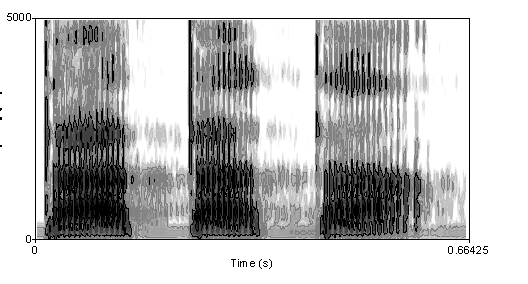
\includegraphics[height=0.3\textheight]{include/spectrogram_example}
	\caption[An example of a spectrogram]{A spectrogram of a male voice saying "ta-ta-ta". Time is shown on the horizontal axis, and frequencies are shown on vertical. The color intensity increases with density. Three separate syllables are clearly visible. Taken from \url{{https://commons.wikimedia.org/}}}
	\label{img:spectrogram_example}
\end{figure}

However, there is a known problem that emerges when windowing is used with the Fourier transform. When the window is rectangular (the wave is cut off vertically from both sides) and is not aligned with the period of the signal, the onset and offset of the wave become abrupt. These sudden changes in amplitude result in the necessity of adding countless additional sine waves to the frequency decomposition, and it begins to contain chaotic information, which makes the valuable parts of the spectrum less precise. An example of this behavior was given in \cite{Schnupp2011} and is shown on the second row of figure \ref{img:windowing_example}.\\

A viable solution of this discontinuity problem comes with attempts to smooth the abrupt ends of the masked wave. Windows that have some kind of ramping on both sides are used in this case. The ramping helps to smoothly turn the sound on and off and reduce the "spectral splatter" \cite{Schnupp2011}. An example of such window (Hanning window) is shown on the third row of figure \ref{img:windowing_example}.\\

\begin{figure}[h]
	\centering
	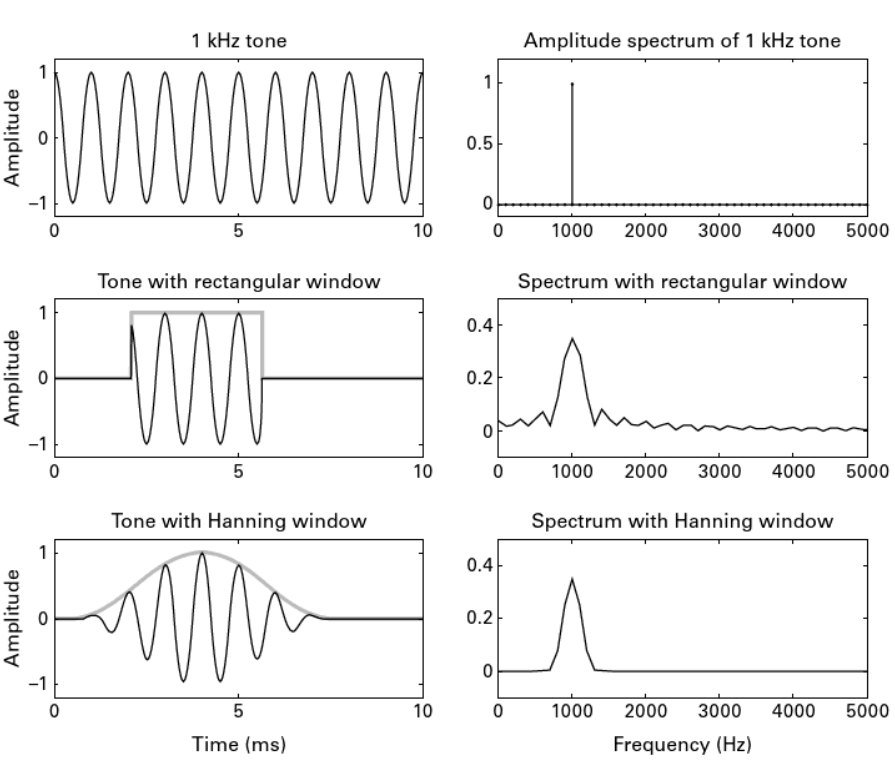
\includegraphics[height=0.5\textheight]{include/windowing_example}
	\caption[An example of windowing and the problem of discontinuities]{The problem of discontinuities that arises when rectangular windows are used. The first row depicts a 1\,kHz pure tone (a sine wave) and its amplitude spectrum. The second row demonstrates the amplitude spectrum of the same tone masked by a rectangular window. The third row shows the spectrum of the same tone masked by a Hanning window. The window functions are shown in gray. Taken from \cite{Schnupp2011}.}
	\label{img:windowing_example}
\end{figure}

It is also worth noticing that when the masking window is short, the resulting amplitude spectrum becomes wider, and vice versa: when the precise frequency representation is needed, the time window must be wide enough. This property is called time-frequency trade-off and can be observed on spectrograms: the spectrograms with high frequency resolution usually have low time resolution, and the ones with high time resolution have low frequency resolution.

\section{Filters and Filterbanks}\label{section:math_filters}

% TODO: impulse response, frequency response
% TODO: SciPy reference
% TODO: IIR and FIR filters
% TODO: filterbanks

\section{Mathematical Concepts used in the Thesis}\label{section:math_concepts}

% TODO: gammatone filter
% TODO: autocorrelation, sacf, cross-channel correlation
% TODO: 
